\section{Introduction to KR}
\begin{itemize}
	\item There are two main lines of development in AI: \textit{symbolic} and \textit{statistical} representation
	\item Both approaches go along with different benefits/weaknesses
	\begin{figure}[ht!]
		\centering
		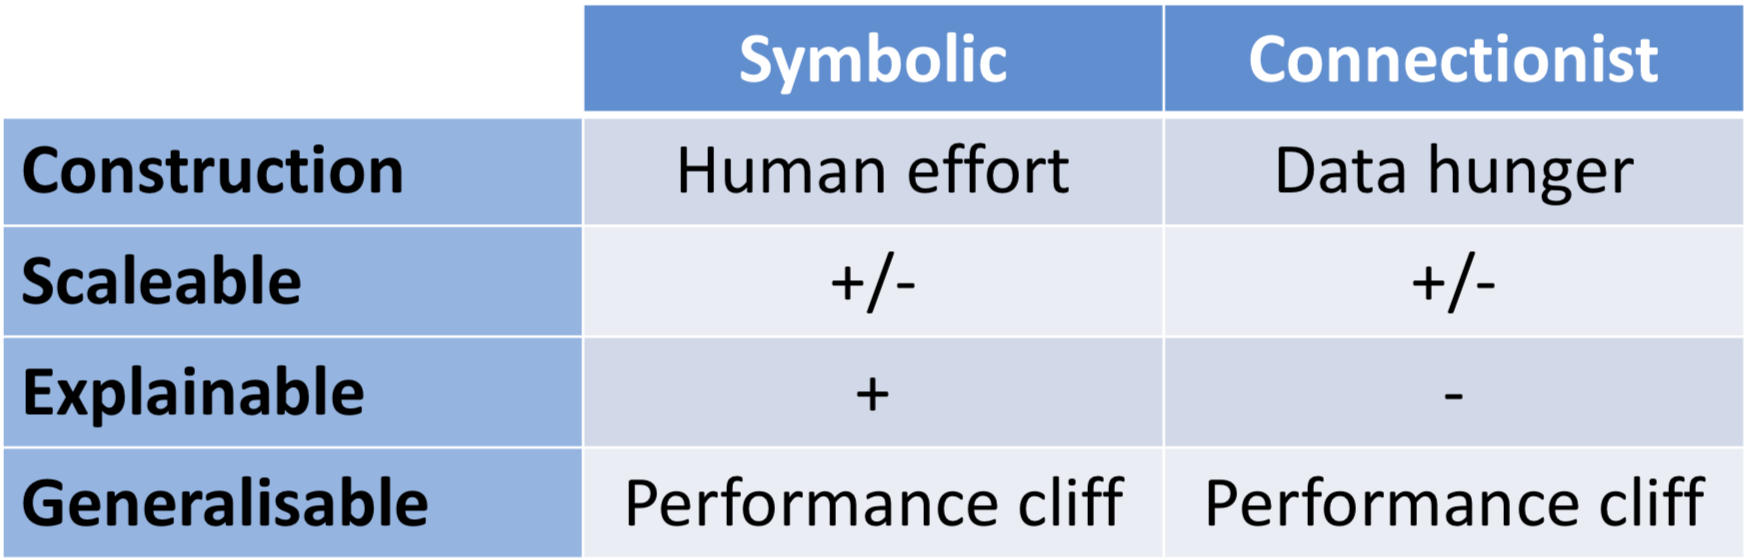
\includegraphics[width=0.5\textwidth]{figures/kr_intro_symbolic_vs_statistical.png}
		\caption{Weaknesses of symbolic and statistical representation in AI}
	\end{figure}
	\begin{itemize}
		\item \textit{\textbf{Construction}}: effort that is needed to create such a system
		\begin{itemize}
			\item A symbolic AI requires a knowledge base on which it bases its reasoning. This knowledge base is mostly created by a human which can take a lot of time. For example, the SNOMED database was created in more than 40 years and contains now about $300,000$ definitions. The construction of knowledge bases is summarized in the research area \textit{Knowledge Engineering}.
			\item In the connectionist/statistical approach, the model learns from data so that we need to provide a (huge) dataset. Depending on the task and the required labels, it can also take a lot of human effort until we have the required data size.
		\end{itemize}
		\item \textit{\textbf{Scalability}}: effect of data size/amount on the systems
		\begin{itemize}
			\item The more data we have for an symbolic AI, the easier it is to run into a problem. Huge knowledge bases tend to be not sound anymore (consistent) as a small mistake at one point can lead to wrong reasoning for any problem (if knowledge base is unsatisfiable, then all given problems are unsatisfiable), So we need to put extra effort in ensuring the soundness of the knowledge base.
			\item Connectionist approaches learn from the statistics of a dataset which gets more accurate by increasing the amount of data. Small errors/noise are thereby smoothed out. However, this also means that statistical representations are inaccurate if there is only a small amount of data. 
		\end{itemize}
		\item \textit{\textbf{Explainable}}: understanding how the system came to its decision
		\begin{itemize}
			\item Symbolic AI is dedicated to creating explainable systems as they only applies facts/statements/rules of the knowledge base that was hand-crafted and thus understandable for a human. The reasoning of such an AI system is explainable by the used and newly derived rules.
			\item In contrast, connectionist approaches are less explainable. As they capture the data distribution in a very high dimensional space (e.g. neural networks with millions of parameters), it more serves as a black box. Errors that are produced by small, carefully selected input noises are harder to understand and to prevent. 
		\end{itemize}
		\item \textit{\textbf{Generalization}}: performance across unseen domains
		\begin{itemize}
			\item Symbolic AI relies on the given knowledge base. If we try to reason about a domain that is unknown in the knowledge base, we don't get any answer (or rather that the reasoning ended without a result). For example, if we have a system based on SNOMED and try to show that if it is raining outside, I probably get wet the AI terminates without an solution because it is not provided by the needed rules/facts.
			\item Commonly, statistical AI systems are already limited to their specific domain. In the task of classification, we usually have a fixed set of classes from which the system has to choose one. If we show a new image that does not belong to any of those, it will try to find the most similar class of what the system has so far (borders in high-dimensional space).
		\end{itemize}
	\end{itemize}
	
\end{itemize}